\section{Pilot Application}

In this network environment, we focus on consumer-facing applications, as shown in Figure~\ref{fig:continuum}. 

\begin{figure*}
\begin{center}
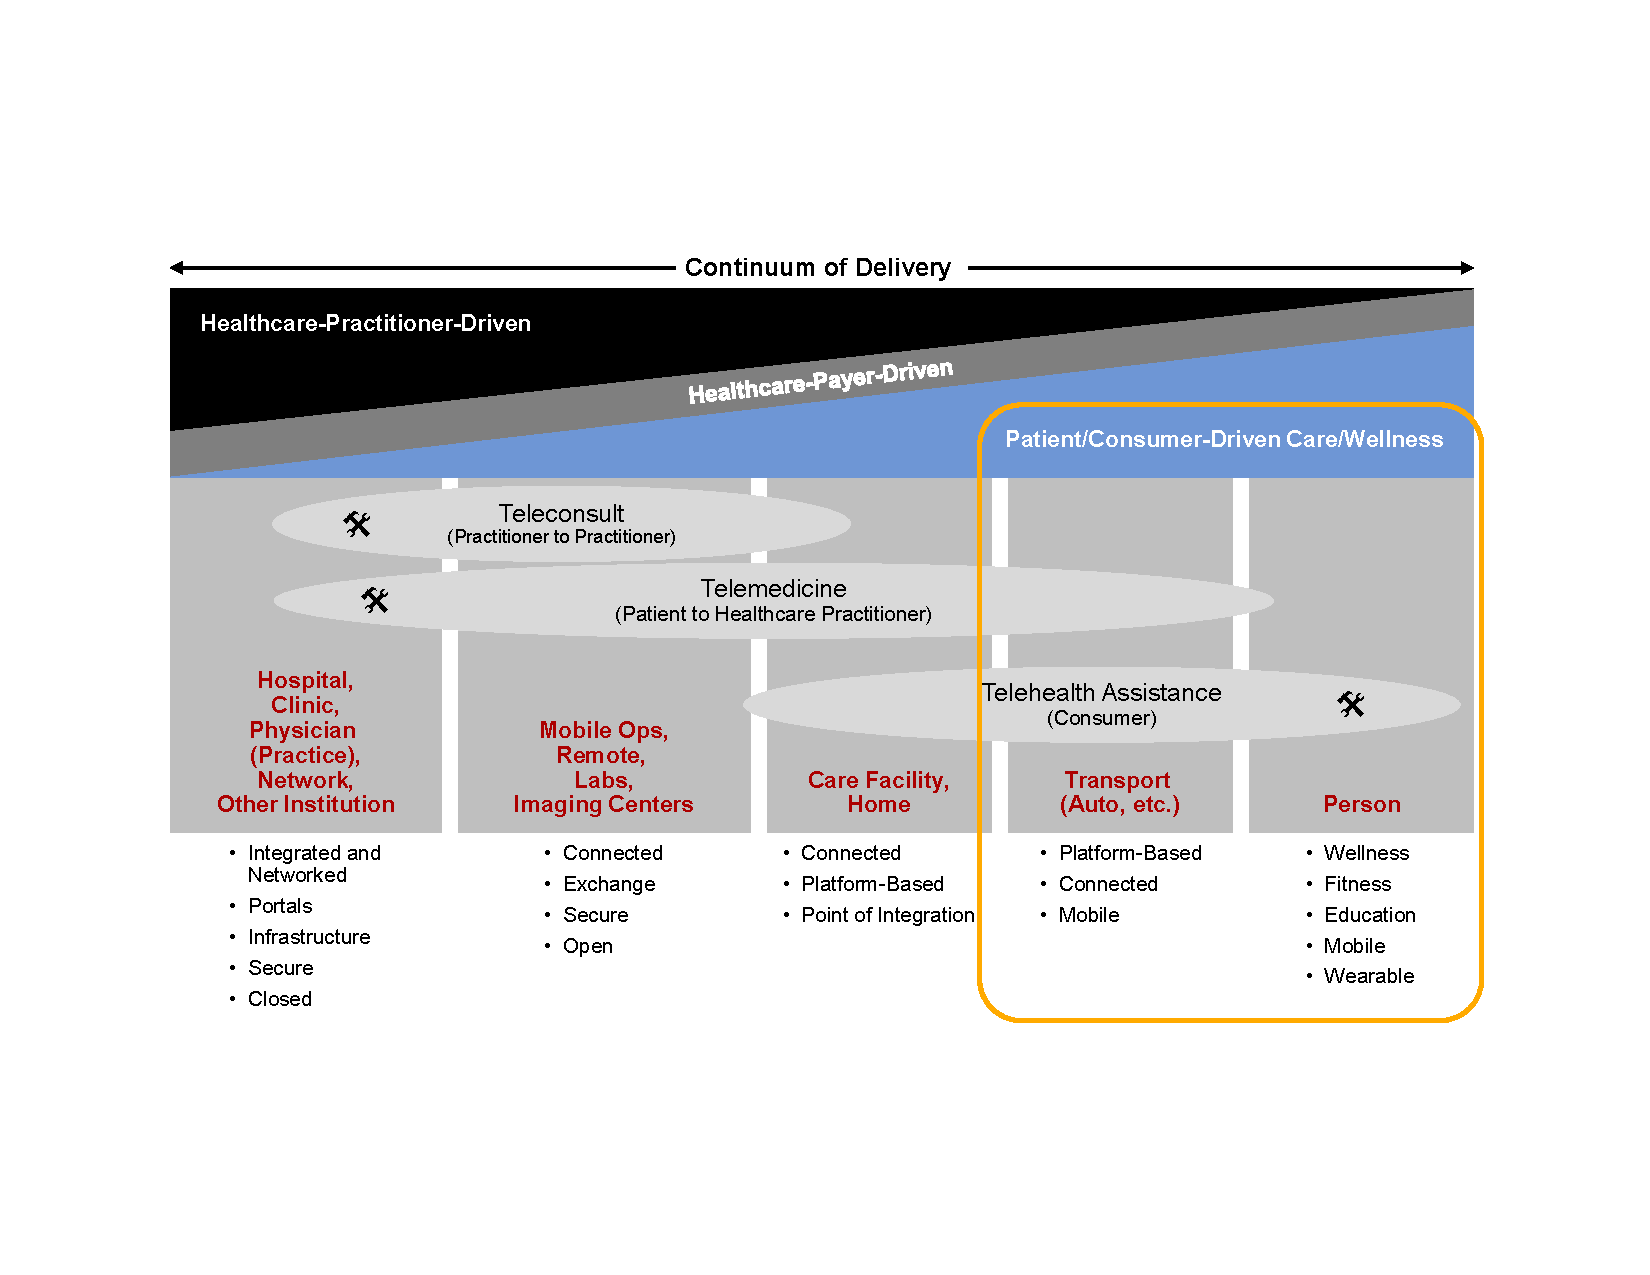
\includegraphics[width=.8\textwidth]{figures/continuum}
\caption{{Focus of Open mHealth network environment shown in yellow box. Figure from Gartner, 2013.  }}
% A Framework for Understanding Telehealth, Telemedicine and Other Remote Healthcare Delivery Solutions
% need to redraw before release
\label{fig:continuum}
\end{center}
\end{figure*}

Our pilot applications:  \textbf{NDNEx} and the required \textbf{Identity Manager}. 

\subsection{Research Requirements} 

{\bf Naming and application design.} The Open mHealth architecture focuses on data exchange rather than system interoperability, which is well-suited for NDN. Using NDN rather than IP enables Open mHealth applications to be coded using data naming directly rather than having to create abstractions to translate data names to IP-based hosts providing services. We will explore how application architecture can be simplified and map closely to network architecture. With its emerging synchronization primitives, NDN will also enhance network support for synchronizing data across multiple devices. 

{\bf Trust and security.} Because NDN does not rely on perimeter- or channel-based security, it will promote global health data ecosystems rather than previous walled garden approaches.   This shift has direct relevance for public health, by enabling research to draw from large populations. 

{\bf Storage in the network.} NDN naturally supports distributed storage, which can ease the burden of fault-tolerance and load-balancing in large networks, reducing cost-of-entry and fostering innovation. 


\subsection{Application Requirements}
The Open mHealth team envisions that the Internet will interconnect 1)
data capture, 2) secure storage, 3) modeling and analytics, and 4) user
interface components to create a modular, layered sense-making framework.  
%% Repeated from above.

Naming and application design
\begin{itemize}
\item What schema? Initially, try direct mapping of Open mHealth schema
\item Borrow ideas from Named Function Networking concept for distributed processing
\item Translate existing REST-based approach or do pure NDN? 
\end{itemize}

Trust and security
\begin{itemize}
\item Replacing Oauth2 for distributed processing is critical
\item Data encryption requirements
\item Name privacy issues
\end{itemize}

Storage in the network
\begin{itemize}
\item Interaction of personal and shared stores
\item Data filtering at the repo?
\item New legal / economic relationship between the players
\end{itemize}